%%%%%%%%%%%%%%%%%%%%%%%%%%%%%%%%%%%%%%%%%%%%%%%%%%%%%%%%%%%%%%%%%%%%%%%
%%%
%%%                東京理科大学 創域理工学部 機械航空宇宙工学科
%%%                   【非公式】卒業論文要旨 テンプレート
%%%
%%%      <https://github.com/tsukahara-lab/TUS-ME_thesis_template>
%%%
%%%                                  v1.3.0 Yuki MATSUKAWA 01 Feb. 2023
%%%                                  v2.0.4 Yuki MATSUKAWA 19 Jan. 2024
%%%                                  v3.0.0 Yuki MATSUKAWA 30 Oct. 2024
%%%
%%%%%%%%%%%%%%%%%%%%%%%%%%%%%%%%%%%%%%%%%%%%%%%%%%%%%%%%%%%%%%%%%%%%%%%

%%% 文書クラスの設定 %%%
\documentclass[
    paper=a4paper,      % A4 用紙サイズ
    article,            % article 相当の文書クラス
    fleqn,              % 数式を左寄せ
    fontsize=12pt,      % 欧文サイズ 12 pt
    jafontsize=12pt,    % 和文サイズ 12 pt
    head_space=20mm,    % 天の余白
    foot_space=15mm,    % 地の余白
    gutter=25mm,        % のどの余白
    fore-edge=10mm,     % 小口の余白
	baselineskip=18pt	% 行送り
    ]{jlreq}            % jlreq クラスを使用

%%% abstract style %%%
% 卒論要旨設定ファイル
\usepackage{settings_bachelor}

% 行番号の表示
% 添削時には行番号を付けるとわかりやすい
% 提出時にはコメントアウトする
\linenumbers

\begin{document}

%%%%%%%%%%%%%%%%%
%%% 日本語要旨 %%%
%%%%%%%%%%%%%%%%%

\begin{center}
\fontsize{16pt}{18pt}\selectfont
\sffamily\bfseries
% 卒業論文の日本語題目
ここには卒業論文のタイトルを入れます.\\ 一文字でも間違えたら受理されません.
% 卒業論文の日本語題目
\end{center}

\noindent
% 姓,名の間に「全角」スペース忘れずに
% 学籍番号と姓の間はスペース不要
% xx を研究室名に変更
% \hfill は消さない
[xx研究室] \hfill 75*****姓姓 名名

\vskip\baselineskip
%%% ここから書き始める %%%

% ダミーテキスト
\jalipsum[1-2]{wagahai}

図~\ref{fig:abst1} は虎,図~\ref{fig:abst2} も虎.

% ダミーテキスト
\jalipsum[3-4]{wagahai}

% 画像は 1, 2 枚程度にしておきましょう.
% 関連する図であれば (a), (b) にしてもいいでしょう.
\begin{figure}[b]
	\centering
	\begin{minipage}{0.35\columnwidth}
		\centering
		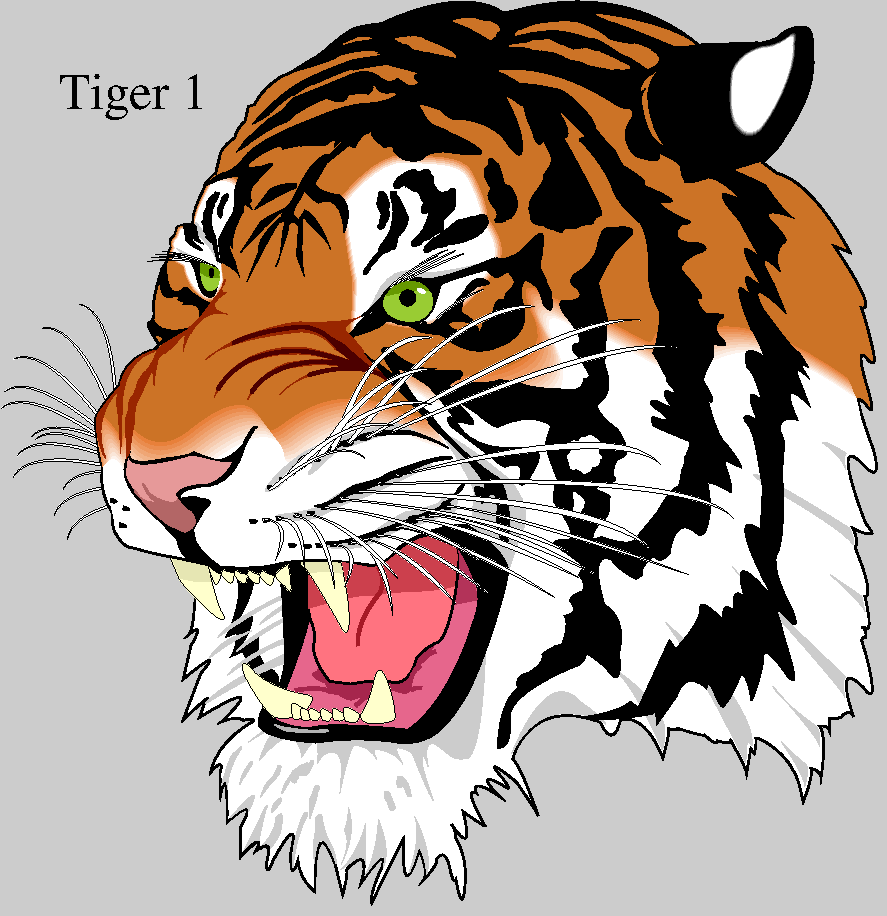
\includegraphics[width=\columnwidth]{tiger1.pdf}
		\caption{Tiger 1.}
		\label{fig:abst1}
	\end{minipage}
	\hspace{15mm}	% 図の間隔は適宜調整
	\begin{minipage}{0.35\columnwidth}
		\centering
		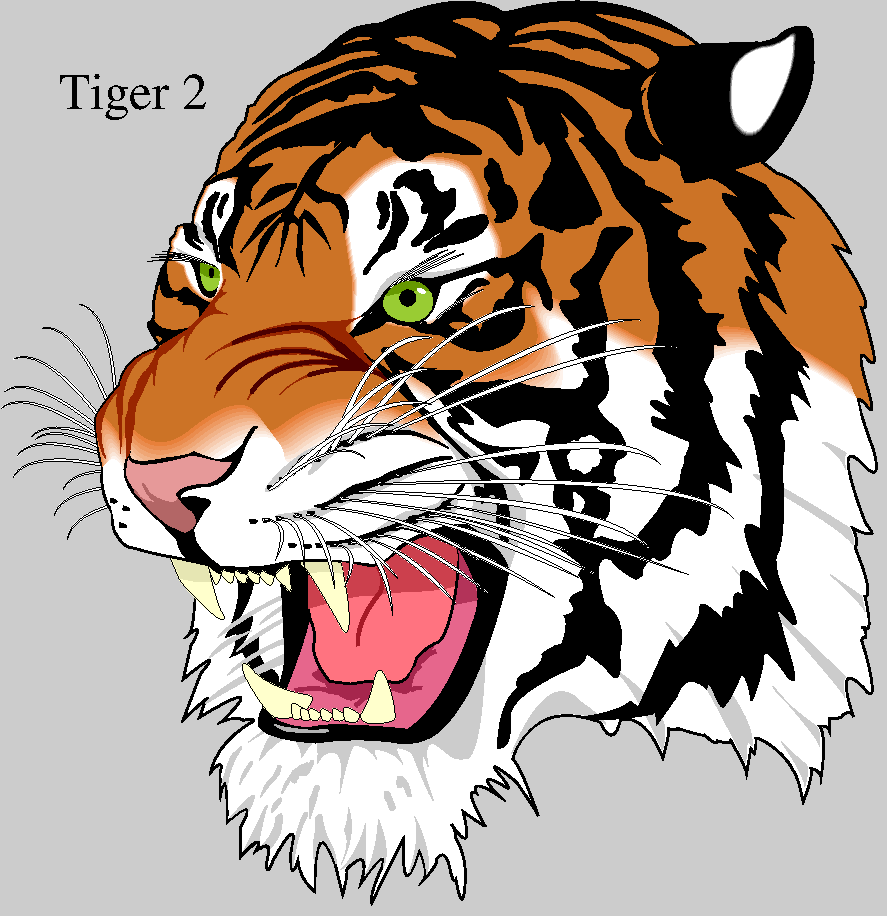
\includegraphics[width=\columnwidth]{tiger2.pdf}
		\caption{Tiger 2.}
		\label{fig:abst2}
	\end{minipage}
\end{figure}

%%% ここまで %%%

%%% ここで改ページ %%%
\clearpage

%%%%%%%%%%%%%%%%%
%%%% 英語要旨 %%%%
%%%%%%%%%%%%%%%%%

\begin{center}
\sffamily\bfseries 
% 卒業論文の英語題目
Enter the title of your graduation thesis here. \\ If you make a mistake in even one letter, it will not be accepted.
% 卒業論文の英語題目
\end{center}

\noindent
% 氏名の大文字小文字に注意(名は冒頭のみ大文字,姓は全て大文字)
% 学籍番号,名,姓の間に「半角」スペース忘れずに
% 英語要旨は日本語要旨と異なり,学籍番号と名の間に半角スペースが必要
% xx を研究室名に変更
% \hfill は消さない
[xx Group] \hfill 75***** First FAMILY

\vskip\baselineskip
%%% ここから書き始める %%%

% ダミーテキスト
\lipsum[1]

%%% ここまで %%%

\end{document}